\documentclass[12pt,a4paper]{article}
\usepackage[utf8]{inputenc}
\usepackage[T1]{fontenc}
\usepackage{authblk}

\usepackage{amsmath, amscd, amsthm, amscd, amsfonts, amssymb, graphicx, color, soul, enumerate, xcolor,  mathrsfs, latexsym, bigstrut, framed, caption}
\usepackage{pstricks,pst-node,pst-tree}
\usepackage[bookmarksnumbered, colorlinks, plainpages,backref]{hyperref}
\hypersetup{colorlinks=true,linkcolor=blue, anchorcolor=green, citecolor=midblue, urlcolor=darkblue, filecolor=magenta, pdftoolbar=true}
\usepackage[all]{xy}

\usepackage{tikz}
%\usetikzlibrary{calc,decorations.pathreplacing,decorations.markings,positioning,shapes}
\usetikzlibrary{calc,decorations.pathreplacing,decorations.markings,positioning,shapes,snakes}

%\usetikzlibrary{calc,decorations.pathreplacing,decorations.markings,positioning,shapes,snakes,external}
%\tikzexternalize

\newcommand{\cp}{\ensuremath{\mathbin{\Box}}}
\newcommand{\Aut}{\ensuremath{\operatorname{Aut}}}
\newcommand{\sym}{\mathrm{Sym}}
\newcommand{\End}{\ensuremath{\operatorname{End}}}
\newcommand{\Prob}{\ensuremath{\operatorname{Pr}}}
\newcommand{\id}{\ensuremath{\text{\rm id}}}
\newcommand{\dist}{\ensuremath{\operatorname{dist}}}
\newcommand{\cg}{\overline{G}}
\newcommand{\D}{\mathrm{D}}
\newcommand{\strong}{\boxtimes}
\newcommand{\supp}{\mathrm{Supp}}
\newcommand\stackplus[1]{\makebox[0ex][l]{$+$} \raisebox{-.75ex}{\makebox[2ex]{$_{#1}$}}}
\newcommand{\rdi}{\mu}
\newcommand {\md}{{\rm mod}\,}
\newcommand\F{F}
\newcommand\Pf{Pf}
%\DeclareMathOperator{\End}{End}
\DeclareMathOperator{\Frob}{Frob}
\def\ld{\mbox{ld}\,}
\definecolor{cupgreen}{rgb}{0,0.498,0.208}
\definecolor{cupblue}{rgb}{0,0,.5}
\definecolor{cupred}{rgb}{1,0.04,0}
\definecolor{cuppink}{rgb}{0.925,0,0.545}
\definecolor{cupmagenta}{rgb}{0.624,0.161,0.424}
\definecolor{cupbrown}{rgb}{0.71,0.212,0.133}

\definecolor{cupgreen}{rgb}{0,0,0}
\definecolor{cupblue}{rgb}{0,0,0}
\definecolor{cupred}{rgb}{0,0,0}
\definecolor{cuppink}{rgb}{0,0,0}
\definecolor{cupmagenta}{rgb}{0,0,0}
\definecolor{cupbrown}{rgb}{0,0,0}

\definecolor{TITLE}{rgb}{0,0,0}
\definecolor{midblue}{rgb}{0.00,0.0,0.80}
\definecolor{darkblue}{rgb}{0.00,0.00,0.45}
\definecolor{SECTION}{rgb}{0.50,0.00,1.00}
\definecolor{THM}{rgb}{0.8,0,0.1}
\definecolor{SEC}{rgb}{0,0,1}
\newcommand{\A}{\mathcal A}
\newcommand{\B}{\mathcal B}
\newcommand{\M}{\mathcal M}
\newcommand{\N}{\mathcal N}
\newcommand{\p}{\mathfrak p}
\newcommand{\q}{\mathfrak q}

\newcommand{\aut}{\mathrm{Aut}}
\newcommand{\m}{\mathrm{M}}
\newcommand{\stab}{\mathrm{Stab}}

\makeatother
\textheight 22truecm \textwidth 17truecm
\setlength{\oddsidemargin}{0.01in}\setlength{\evensidemargin}{0.01in}
\renewcommand{\baselinestretch}{1.05}\normalsize
\newtheorem{theorem}{{\color{THM} Theorem}}[section]
\newtheorem{procedure}{{\color{THM} Procedure}}[section]
\setlength{\topmargin}{-.2cm}


\DeclareRobustCommand{\stirling}{\genfrac\{\}{0pt}{}}

\newtheorem{lemma}[theorem]{{\color{THM}Lemma}}
\newtheorem{proposition}[theorem]{{\color{THM}Proposition}}
\newtheorem{corollary}[theorem]{{\color{THM}Corollary}}
\newtheorem{conjecture}[theorem]{{\color{THM}Conjecture}}
\theoremstyle{definition}
\newtheorem{definition}[theorem]{{\color{THM}Definition\ }}
\newtheorem{question}[theorem]{{\color{THM}Question\ }}
\newtheorem{example}[theorem]{{\color{THM}Example}}
\newtheorem{examples}[theorem]{{\color{THM}Examples}}
\newtheorem{xca}[theorem]{{\color{THM}Exercise}}
\newtheorem{problem}[theorem]{{\color{THM}Problem}}
\newtheorem{remark}[theorem]{{\color{THM}Remark}}
\numberwithin{equation}{section}

\renewcommand{\refname}{{\color{SEC} References}}
\newcommand{\f}{\rightarrow}
\newcommand{\la}{\langle}
\newcommand{\ra}{\rangle}
\date{}


\title{Response to a review on\\
{\bf Noncontextual coloring of orthogonality hypergraphs}}


\author{}
%\author[1]{Mohammad H. Shekarriz\thanks{mhshekarriz@yazd.ac.ir}}

%\affil[1]{Department of Mathematics, Yazd University, 89195-741, Yazd, Iran.}

%\author[2]{Karl Svozil\thanks{svozil@tuwien.ac.at, %http://tph.tuwien.ac.at/$\sim$svozil}}

%\affil[2]{Institute for Theoretical Physics,
%       Vienna  University of Technology,
%       Wiedner Hauptstrasse 8-10/136,
%       1040 Vienna,  Austria}


\begin{document}

        \maketitle

        We would like to thank the Referee for the valuable criticism and suggestions brought forward. We have revised the manuscript accordingly, as outlined below. In what follows we also respond by mentioning some specific arguments that are pertinent but need not be included in the main text.

        Note that references here are made to the previous version of the paper. The new version is called ``the revised version''.

\begin{quotation}
        (*1) {\it ``It is difficult to recognize the contribution of the paper from the text.''}
\end{quotation}

We added some paragraphs in the first section explaining the contribution of the paper. Moreover, we altered the abstract, restructured some sections and modified the conclusion.

\begin{quotation}
        (*2) {\it ``In the proposed simple counterexample to Conjecture 4, the hypergraph is separable (that was needed) and it seems that it is not reconstructable.
        There may be a misunderstanding in the basic definition of a ``reconstructable hypergraph'', which is missing!''}
\end{quotation}

Reconstruction is an old concept in graph theory, for example we can mention the famous 70-year-old reconstruction conjecture of Kelly and Ulam. The proposed hypergraph shows that the reviewer has fully understood this concept. Anyway, we added a sentence in the paper to prevent any sense of ambiguity.

If the coiled-shape edges in the proposed hypergraph replaced with the Specker bug, it has 121 two-valued states and is reconstructable using the adjacency criterion (Criterion 6) and the completion criterion (Criterion 2). In fact this hypergraph is very similar to the hypergraph depicted in Figure 2 (in the paper). Let us have a closer look.

We drew the proposed hypergraph in Figure~\ref{fig:proposed} (I) here. Similar to the hypergraph of Figure 2 of the paper, when we use only Criterion 6, we reconstruct it as the hypergraph depicted in Figure~\ref{fig:proposed} (II). This is because when $a$ is true, $g$ and $s$ have to be both false. Similarly, when $g$ is true, $a$ and $s$ have to be false and when $s$ is true, both $a$ and $g$ have to be false. This is like $a$, $g$ and $s$ lie on a context.

If there were a context containing $a$, $g$ and $s$, then in any two-valued state at least one of them has to be assigned 1. However, there are two-valued states that assign 0 to all of them. Therefore, if one uses the two criteria 2 and 6 at the same time, he understand that there must not be a context containing $a$, $g$ and $s$. So, he reconstructs it like Figure~\ref{fig:proposed} (III) which is identical to the original proposed hypergraph. Consequently, the proposed hypergraph is reconstructable and is not a counterexample for Conjecture 4.

Although we have stated this several times in the paper that for a context every two-valued state assigns 1 to only one vertex and 0 to others, we added this again to a paragraph after the completion criterion in the revised version, in order to prevent any further ambiguity.

        \begin{figure}
        \begin{center}
                \begin{tabular}{ c c c c c }

                        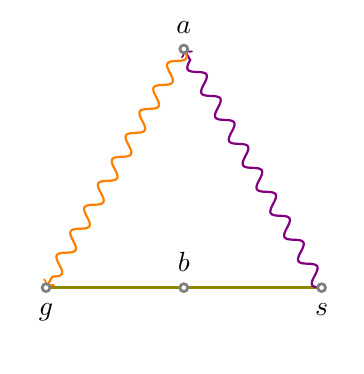
\begin{tikzpicture} [scale=0.35]

                                \tikzstyle{every path}=[line width=1pt]

                                \newdimen\ms
                                \ms=0.15cm
                                \tikzstyle{s1}=[color=black,fill,rectangle,inner sep=3]
                                \tikzstyle{c1}=[draw=gray,fill=white,circle,inner sep={1}]

                                % Define positions of all observables



                                \coordinate (a7) at (-4,-3);
                                \coordinate (a8) at (6,-3);
                                \coordinate (a9) at (1,5.6602);
                                \coordinate (a10) at (1,-3);
                                % draw contexts



                                \draw [color=olive,] (a7) -- (a8);
                                \draw [color=violet, ->,snake=coil,segment aspect=0,thick] (a8) to node[right] { } (a9);
                                \draw [color=orange, ->,snake=coil,segment aspect=0,thick] (a9) to node[left] { } (a7);




                                % draw atoms


                                \draw (a7) coordinate[c1,label=below:$g$];
                                \draw (a8) coordinate[c1,label=below:$s$];
                                \draw (a9) coordinate[c1,label=above:$a$];
                                \draw (a10) coordinate[c1,label=above:$b$];
                        \end{tikzpicture}

                        & \hspace{0.6 cm} &

                        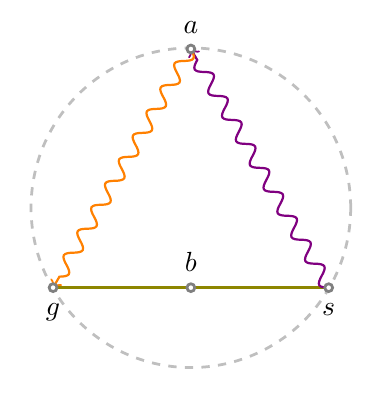
\begin{tikzpicture} [scale=0.35]

                                \tikzstyle{every path}=[line width=1pt]

                                \newdimen\ms
                                \ms=0.15cm
                                \tikzstyle{s1}=[color=black,fill,rectangle,inner sep=3]
                                \tikzstyle{c1}=[draw=gray,fill=white,circle,inner sep={1}]
%                               \tikzstyle{every tto}=[draw,dashed]


                                % Define positions of all observables



                                \coordinate (a7) at (-4,-3);
                                \coordinate (a8) at (6,-3);
                                \coordinate (a9) at (1,5.6602);
                                \coordinate (a10) at (1,-3);
                                % draw contexts



                                \draw [color=olive] (a7) -- (a8);
                                \draw [color=violet, ->,snake=coil,segment aspect=0,thick] (a8) to node[right] { } (a9);
                                \draw [color=orange, ->,snake=coil,segment aspect=0,thick] (a9) to node[left] { } (a7);
                                \draw [color=lightgray,dashed] (1,-0.1) circle (165pt);

                        %       \draw [color=lightgray] (-4,-3) .. controls (-1,0.555) and (-0.555,1) .. (6,-3) .. controls (0.555,1) and (1,0.555) .. (1,5.6602)                       .. controls (0.555,1) and (1,0.555) .. (-4,-3);




                                % draw atoms


                                \draw (a7) coordinate[c1,label=below:$g$];
                                \draw (a8) coordinate[c1,label=below:$s$];
                                \draw (a9) coordinate[c1,label=above:$a$];
                                \draw (a10) coordinate[c1,label=above:$b$];
                        \end{tikzpicture}

                        & \hspace{0.6 cm} &

                        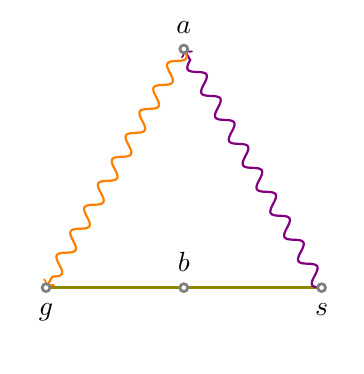
\begin{tikzpicture} [scale=0.35]

                                \tikzstyle{every path}=[line width=1pt]

                                \newdimen\ms
                                \ms=0.15cm
                                \tikzstyle{s1}=[color=black,fill,rectangle,inner sep=3]
                                \tikzstyle{c1}=[draw=gray,fill=white,circle,inner sep={1}]

                                % Define positions of all observables



                                \coordinate (a7) at (-4,-3);
                                \coordinate (a8) at (6,-3);
                                \coordinate (a9) at (1,5.6602);
                                \coordinate (a10) at (1,-3);
                                % draw contexts



                                \draw [color=olive,] (a7) -- (a8);
                                \draw [color=violet, ->,snake=coil,segment aspect=0,thick] (a8) to node[right] { } (a9);
                                \draw [color=orange, ->,snake=coil,segment aspect=0,thick] (a9) to node[left] { } (a7);




                                % draw atoms


                                \draw (a7) coordinate[c1,label=below:$g$];
                                \draw (a8) coordinate[c1,label=below:$s$];
                                \draw (a9) coordinate[c1,label=above:$a$];
                                \draw (a10) coordinate[c1,label=above:$b$];
                        \end{tikzpicture}

                        \\

                        (I)&&(II)&&(III)
                \end{tabular}
        \end{center}
        \caption{\label{fig:proposed}
                The proposed hypergraph (I), reconstruction of it via only Criterion 6 (II) and its reconstruction via Criteria 2 and 6 (III). The dashed context (gray circle) in (II) disappears when we use the completion criterion because there are two-valued states that assign 0 to all $a$, $g$ and $s$.}
\end{figure}

By using the proposed hypergraph, we maybe be able to construct another, extended, hypergraph, based on the proposed one, such that the new one is not reconstructable using criteria 2 and 6. But due to its similarity with the hypergraph of Figure 2 in the paper, it seems that  the same amount of work is required to show that the new hypergraph is separable but is not reconstructable.


\begin{quotation}
        (*3) {\it ``Is the condition 4 of Definition 5 needed? I suppose not.

        Just apply condition 1 to $a_i$ and some $a_k$ adjacent to $a_j$, provided that such a $k$ exists.''}
\end{quotation}

We agree that the condition 4 of Definition 5 is a result of conditions 1 or 3. Therefore, we altered Definition 5, a paragraph after Definition 5, and the proof of Theorem 7 in the paper accordingly.

\begin{quotation}
         (*4) {\it ``This may require, as mentioned in the first review, to check if your results are correctly formulated also for hypergraphs with small edges, with 1 or 2 elements.''}
\end{quotation}

We added a paragraph dedicated to hypergraphs whose hyperedges consist of 1 or 2 vertices.

\begin{quotation}
        (*5) {\it``Criterion 6 should start with a capital letter.''}

        (*6) {\it ``The caption of Figure 9 should refer to Figure 3 to explain what are ``the nine $G_i$'s''.''}
\end{quotation}

We have done both of these corrections accordingly. We would like to thank the Referee again for the attention dedicated to the manuscript, and for the valuable criticism and suggestions.

\end{document}
